%% Elsevier single-column manuscript draft.
%% Numerical results labelled "illustrative" are synthetic layout placeholders.
\documentclass[a4paper,fleqn]{cas-sc}

\usepackage[authoryear,longnamesfirst]{natbib}
\usepackage{amsmath}
\usepackage{amssymb}
\usepackage{array}
\usepackage{float}
\usepackage{placeins}
\usepackage{booktabs}
\usepackage{multirow}
\usepackage{xcolor}
\usepackage{tikz}
\usetikzlibrary{arrows.meta,positioning,fit}
\usepackage{pgfplots}
\usepgfplotslibrary{groupplots}
\pgfplotsset{compat=1.18}

%%% Author macros
\def\tsc#1{\csdef{#1}{\textsc{\lowercase{#1}}\xspace}}
\tsc{WGM}
\tsc{QE}

\ExplSyntaxOn
\keys_set:nn { stm / mktitle } { nologo }
\cs_set:Npn \__first_footerline:
{
    \group_begin:
    \small
    \sffamily
    \ifnum\theblind>0\relax
    \else
        \__short_authors:
    \fi
    \group_end:
}
\ExplSyntaxOff

\definecolor{DeepTeal}{HTML}{264653}
\definecolor{MineralGreen}{HTML}{2A9D8F}
\definecolor{MutedAmber}{HTML}{E9C46A}
\definecolor{WarmSand}{HTML}{F4A261}
\definecolor{CoralRust}{HTML}{E76F51}
\definecolor{MutedPlum}{HTML}{6D597A}
\definecolor{SteelBlue}{HTML}{577590}
\definecolor{DraftCream}{HTML}{FFF7E6}
\newcommand{\illustrative}{\textsuperscript{\textcolor{CoralRust}{\textbf{I}}}}

\begin{document}
\let\WriteBookmarks\relax
\def\floatpagepagefraction{1}
\def\textpagefraction{.001}

% Keep author-identifying metadata blank here until the final submission stage.
\shorttitle{Model-Agnostic Physical Enforcement in Tabular Surrogates}
\shortauthors{}

\title[mode=title]{Model-Agnostic Enforcement of Mass Conservation and Non-Negativity in Tabular Surrogates of Activated Sludge Processes}

\author{}

\begin{abstract}
Artificial intelligence and machine-learning tools are increasingly used as fast surrogates for activated-sludge simulation, yet wastewater studies have largely judged these models by predictive accuracy without requiring physically admissible outputs. To our knowledge, this work is designed as the first demonstration, for tabular surrogates of an activated-sludge process, of a model-agnostic post-prediction method that simultaneously enforces mass conservation and componentwise non-negativity. We transfer the positivity-preserving conservative projection of Kircher and Votsmeier to steady-state effluent prediction; we do not introduce a new projection algorithm. Nine tabular learners spanning boosting, bagging, kernel, neighbor, latent-variable, and neural-network methods map operating conditions and influent composition to a 20-component effluent state. Supporting analyses use five-fold cross-validation across eleven dataset sizes, computational timing, and separately simulated inputs beyond the training envelope. \textit{The numerical findings currently shown are explicit placeholders pending execution of the complete benchmark.} The final analysis will quantify how enforcement changes predictive error while verifying conservation and non-negativity within numerical tolerance. The study separates the guaranteed physical contract from empirical predictive performance and applies the same correction to heterogeneous predictors without retraining.
\end{abstract}

\begin{graphicalabstract}
\centering
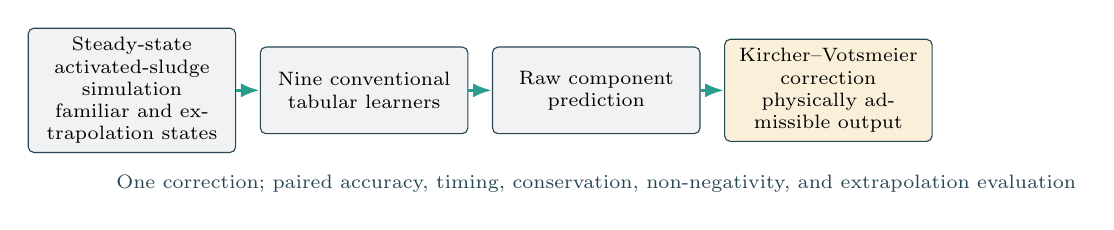
\begin{tikzpicture}[
  node distance=3mm,
  box/.style={draw=DeepTeal, rounded corners=2pt, fill=DeepTeal!7,
              minimum height=11mm, text width=24mm, align=center, font=\scriptsize},
  arrow/.style={-{Latex[length=2.4mm]}, very thick, draw=MineralGreen}
]
\node[box] (sim) {Steady-state activated-sludge simulation\\familiar and extrapolation states};
\node[box, right=of sim] (ml) {Nine conventional\\tabular learners};
\node[box, right=of ml] (split) {Raw component\\prediction};
\node[box, right=of split, fill=MutedAmber!25] (proj) {Kircher--Votsmeier correction\\physically admissible output};
\draw[arrow] (sim) -- (ml);
\draw[arrow] (ml) -- (split);
\draw[arrow] (split) -- (proj);
\node[align=center, font=\scriptsize, text=DeepTeal, below=4mm of split] {One correction; paired accuracy, timing, conservation, non-negativity, and extrapolation evaluation};
\end{tikzpicture}
\end{graphicalabstract}

\begin{highlights}
\item A model-agnostic correction enforces mass conservation and non-negativity together.
\item The benchmark is designed as the first such activated-sludge demonstration.
\item Nine conventional learners test applicability across heterogeneous model classes.
\item Data scarcity, computation, and extrapolation will be assessed alongside accuracy.
\item The analysis separates guaranteed physical validity from predictive performance.
\end{highlights}

\begin{keywords}
activated sludge model \sep surrogate modeling \sep tabular machine learning \sep mass conservation \sep non-negativity
\end{keywords}

\maketitle

\begin{center}
\fcolorbox{CoralRust}{DraftCream}{%
\parbox{0.92\textwidth}{\small\textbf{Draft-results notice.}
All numerical values marked with \illustrative, and every figure or table whose caption begins ``Illustrative'', are synthetic results included to demonstrate the intended analysis and presentation. They must be replaced by outputs from the final benchmark before scientific submission.}}
\end{center}

\section*{Nomenclature}
\begin{tabbing}
\hspace{3.9cm} \= \kill
ASM \> Activated Sludge Model \\
ASM2d-TSN \> Activated Sludge Model No.\ 2d with two-step nitrification \\
$A$ \> Full-row-rank invariant matrix defining the ASM conservation constraints \\
$b_i$ \> Conservation target for sample $i$, $b_i = A c_{in,i}$ \\
$c$ \> Generic ASM component concentration vector \\
$c_+$ \> Strictly positive scaling target, $c_+ = \max(c_{raw},\varepsilon\mathbf{1})$ componentwise \\
$c_{in}$ \> Influent ASM component concentration vector \\
$c_{out}$ \> True steady-state effluent ASM component concentration vector \\
$c_{raw}^{(m)}$ \> Raw effluent component prediction from surrogate model $m$ \\
$c_{cand}^{(m)}$ \> Conservative candidate before positivity backtracking \\
$\tilde{c}^{(m)}$ \> Projected effluent component prediction from surrogate model $m$ \\
$q^*$ \> Least-squares coordinates of the conservative correction in the basis $Z$ \\
$d_c^{*,(m)}$ \> Standardized component-space displacement caused by projection \\
$\varepsilon$ \> Positive lower bound used in projection scaling; $10^{-8}$ \\
$\eta$ \> Numerical safety margin used by positivity backtracking \\
$F$ \> Number of ASM component targets; $F=20$ in this study \\
$f_m$ \> Already trained tabular surrogate model $m$ \\
$I_{comp}$ \> Matrix mapping ASM components to reported effluent composites \\
$N$ \> Total number of observations at a data-scarcity scale \\
$n$ \> Number of observations in a scored validation fold \\
$r$ \> Number of independent conservation constraints; $r=5$ \\
$s$ \> Componentwise inverse scaling vector, $s=1/c_+$ \\
$\sigma_j$ \> Training-fold standard deviation of component $j$ \\
$\tau$ \> Numerical tolerance used to classify physical violations \\
$u$ \> Operating-variable vector \\
$v_{mc}$ \> Mass-conservation residual for a component prediction \\
$v_{nn}^{*}$ \> Standardized non-negativity violation magnitude \\
$W_s$ \> Diagonal scaling matrix, $W_s=\mathrm{Diag}(s)$ \\
$y$ \> Reported effluent-quality composite vector \\
$y_{raw}^{(m)}$ \> Reported composite vector computed from $c_{raw}^{(m)}$ \\
$\tilde{y}^{(m)}$ \> Reported composite vector computed from $\tilde{c}^{(m)}$ \\
$Z$ \> Orthonormal basis for the null space of $A$ used in this manuscript \\
$\nu$ \> Stoichiometric/Petersen matrix for the ASM2d-TSN process model \\
$\alpha_i$ \> Positivity-preserving backtracking factor for sample $i$ \\
$\mathcal{F}_i$ \> Feasible component set for sample $i$ \\
$\odot$ \> Elementwise multiplication \\
$\oslash$ \> Elementwise division \\
$\top$ \> Matrix transpose \\
COD \> Chemical oxygen demand \\
CSTR \> Continuous stirred tank reactor \\
HRT \> Hydraulic retention time \\
MLP \> Multilayer perceptron \\
nMAE \> Component-standardized aggregate mean absolute error \\
nMSE \> Component-standardized aggregate mean squared error \\
nRMSE \> Component-standardized aggregate root mean squared error \\
OOD \> Out-of-distribution \\
PAO \> Phosphate-accumulating organisms \\
PLS \> Partial least squares \\
$R^2$ \> Coefficient of determination \\
SVR \> Support vector regression \\

ID \> In-distribution \\
TN \> Total nitrogen \\
TP \> Total phosphorus \\
TSS \> Total suspended solids \\
\end{tabbing}

\section{Introduction}

Water pollution remains a major environmental and public-health challenge. Activated-sludge systems are central to biological wastewater treatment because they remove carbon, nitrogen, phosphorus, and suspended solids through coupled microbial and physicochemical transformations (Duan et al., 2022; Lin et al., 2022; Madhav et al., 2019). Activated Sludge Models (ASM) provide a mechanistic description of these transformations, but their nonlinear reaction networks can make repeated simulation, design, and optimization expensive (Aboagye et al., 2021; Henze et al., 2006; Padron-Paez et al., 2020; Xiao et al., 2025).

Surrogate models offer faster approximations of this mechanistic behavior (Bhosekar \& Ierapetritou, 2018; Durkin et al., 2024; Tsochatzidi et al., 2025). Wastewater applications now include linear and kernel methods, tree ensembles, and neural networks (Ahn et al., 2014; Asadi et al., 2017; Bagherzadeh et al., 2021; Mao et al., 2024; Wang et al., 2025). The rapid adoption of artificial intelligence and machine-learning tools makes physical safeguards increasingly important: faster prediction is useful only when the predicted state remains meaningful.

Predictive accuracy alone does not guarantee a physically admissible activated-sludge state. Conservation and non-negativity apply to the underlying component vector before it is converted into chemical oxygen demand (COD), total nitrogen (TN), total phosphorus (TP), and total suspended solids (TSS). A surrogate can therefore approximate these reported quantities while violating material inventories or predicting negative concentrations. Either failure can mislead process interpretation, optimization, monitoring, or design. A prediction that conserves mass but contains a negative component is no more usable than a non-negative prediction that creates or destroys a conserved inventory.

This dual requirement has remained largely absent from the wastewater surrogate literature, which has generally emphasized predictive error (Bagherzadeh et al., 2021; Mao et al., 2024; Wang et al., 2025; Yang et al., 2025). Conservation-aware methods exist in other scientific domains, including analytic constraints, conservative architectures, and post-prediction reconciliation (Beucler et al., 2021; Hansen et al., 2024; Sturm \& Wexler, 2020, 2022). Yet conservation-only correction can still produce negative components, while clipping or positive output transformations can destroy conservation. Soft penalties can encourage both properties but generally do not guarantee them at deployment (Raissi et al., 2019; Hansen et al., 2024).

Kircher and Votsmeier (2025) address both requirements with a scaled, conservation-preserving projection followed by positivity backtracking. Their correction acts on a completed component prediction, so it does not depend on the internal architecture, objective, or gradients of the model that produced that prediction. Related work confirms that simultaneous conservation and positivity are mathematically achievable in other settings (Sturm et al., 2023; Min et al., 2024; Utkarsh et al., 2025). What has remained untested is whether this model-agnostic strategy can provide the same physical contract across heterogeneous tabular surrogates of an activated-sludge process.

To our knowledge, this study is designed as the first demonstration of model-agnostic, simultaneous enforcement of mass conservation and componentwise non-negativity across tabular surrogates for an activated-sludge process. The benchmark will transfer and systematically evaluate the Kircher--Votsmeier correction; it does not claim a new projection algorithm or a new learning model. The intended primary contribution is the activated-sludge demonstration itself, which addresses a long-overlooked requirement that becomes more consequential as artificial intelligence and machine-learning tools enter environmental modeling workflows.

The benchmark is designed to provide supporting evidence for that contribution. Nine conventionally fitted learners predict the 20-component steady-state effluent of a continuous stirred tank reactor. The final analysis will measure predictive accuracy, data-scarcity stability, training and inference cost, conservation residuals, negative components, and performance on inputs beyond the training envelope. The shared post-prediction interface allows the physical correction to be evaluated independently of model architecture.

\section{Methods}

\subsection{Simulated Activated Sludge Process and Dataset Generation}

The in-distribution (ID) benchmark data were generated with a standalone, steady-state continuous stirred tank reactor (CSTR). The reactor was represented by Activated Sludge Model No.\ 2d with two-step nitrification (ASM2d-TSN). This model contains 20 components and 28 coupled processes spanning hydrolysis, heterotrophic and phosphate-accumulating-organism metabolism, two-step nitrification and denitrification, lysis, and precipitation--redissolution. The model basis follows Henze et al. (2006), while the two-step nitrification formulation, stoichiometry, and rate coefficients follow Guerrero et al. (2011).

The dissolved components are dissolved oxygen ($S_O$), fermentable substrate ($S_F$), acetate ($S_A$), ammonium nitrogen ($S_{NH4}$), nitrite nitrogen ($S_{NO2}$), nitrate nitrogen ($S_{NO3}$), dinitrogen ($S_{N2}$), soluble phosphate ($S_{PO4}$), soluble inert organic matter ($S_I$), and alkalinity ($S_{ALK}$). The particulate components are particulate inert organic matter ($X_I$), slowly biodegradable substrate ($X_S$), heterotrophic biomass ($X_H$), phosphate-accumulating-organism biomass ($X_{PAO}$), stored polyphosphate ($X_{PP}$), stored polyhydroxyalkanoates ($X_{PHA}$), ammonia-oxidizing biomass ($X_{AOB}$), nitrite-oxidizing biomass ($X_{NOB}$), precipitated metal phosphate ($X_{MeP}$), and metal hydroxide ($X_{MeOH}$).

Every evaluated method produces this same 20-component effluent state. Chemical oxygen demand, total nitrogen, total phosphorus, and total suspended solids are calculated afterward as $y=I_{comp}c$. The matrix $I_{comp}$ supplies one common component-to-reporting map for all raw and projected predictions; the models are not fitted directly to the four reported composites.

The simulation design sampled 22 inputs: hydraulic retention time (HRT), aeration, and the 20 influent component concentrations. Latin hypercube sampling with random seed 42 continued until 10,000 valid steady-state samples were accepted. Table~\ref{tab:simulation_domain} lists the sampled domain. These bounds define the familiar operating and influent envelope used for the ID analysis.

\begin{table}[htbp]
\centering
\caption{Sampled operating and influent variables used to generate the steady-state Activated Sludge Model No.\ 2d with two-step nitrification (ASM2d-TSN) dataset.}
\label{tab:simulation_domain}
\scriptsize
\setlength{\tabcolsep}{3pt}
\begin{tabular}{p{2.1cm}p{2.7cm}p{2.8cm}p{3.0cm}}
\hline
Variable & Category & Range & Unit \\
\hline
$\mathrm{HRT}$ & Operating & [6.0, 36.0] & h \\
$\mathrm{Aeration}$ & Operating & [0.5, 2.5] & -- \\
$S_O$ & Influent dissolved & [0.0, 0.5] & g O$_2$/m$^3$ \\
$S_F$ & Influent dissolved & [20.0, 180.0] & g COD/m$^3$ \\
$S_A$ & Influent dissolved & [5.0, 80.0] & g COD/m$^3$ \\
$S_{NH4}$ & Influent dissolved & [12.0, 55.0] & g N/m$^3$ \\
$S_{NO2}$ & Influent dissolved & [0.0, 3.0] & g N/m$^3$ \\
$S_{NO3}$ & Influent dissolved & [0.0, 8.0] & g N/m$^3$ \\
$S_{N2}$ & Influent dissolved & [0.0, 2.0] & g N/m$^3$ \\
$S_{PO4}$ & Influent dissolved & [2.0, 18.0] & g P/m$^3$ \\
$S_I$ & Influent dissolved & [10.0, 90.0] & g COD/m$^3$ \\
$S_{ALK}$ & Influent dissolved & [80.0, 260.0] & mol/m$^3$ \\
$X_I$ & Influent particulate & [20.0, 120.0] & g COD/m$^3$ \\
$X_S$ & Influent particulate & [60.0, 280.0] & g COD/m$^3$ \\
$X_H$ & Influent particulate & [15.0, 100.0] & g COD/m$^3$ \\
$X_{PAO}$ & Influent particulate & [5.0, 60.0] & g COD/m$^3$ \\
$X_{PP}$ & Influent particulate & [2.0, 20.0] & g P/m$^3$ \\
$X_{PHA}$ & Influent particulate & [1.0, 30.0] & g COD/m$^3$ \\
$X_{AOB}$ & Influent particulate & [0.5, 8.0] & g COD/m$^3$ \\
$X_{NOB}$ & Influent particulate & [0.5, 8.0] & g COD/m$^3$ \\
$X_{MeP}$ & Influent particulate & [0.0, 12.0] & g TSS/m$^3$ \\
$X_{MeOH}$ & Influent particulate & [0.0, 12.0] & g TSS/m$^3$ \\
\hline
\end{tabular}
\end{table}

For each sampled input, nonlinear least squares solved the steady-state balance equations under state bounds of $10^{-8}$ and 1500. Variable, residual, and gradient tolerances were $10^{-9}$, and each solve was limited to 1200 function evaluations. Up to 25 candidate attempts were allowed for each accepted sample. Two physically informed initializations were tried first. If both failed, the process was dynamically relaxed for 20 days with a stiff backward differentiation formula (BDF) integrator, and its terminal state became a new steady-state guess. Only converged states with maximum absolute residual no greater than $10^{-9}$ were retained. The 28 mechanistic process rates were evaluated from the ASM2d-TSN kinetics without an artificial rate ceiling or rate clipping; the stated bounds apply to solved state variables, not to reaction rates.

\begin{table}[htbp]
\centering
\caption{Simulation and acceptance settings used to construct the benchmark dataset.}
\label{tab:simulation_settings}
\scriptsize
\begin{tabular}{p{3.7cm}p{7.2cm}}
\hline
Setting & Value or rule \\
\hline
Process model & Standalone steady-state continuous stirred tank reactor based on ASM2d-TSN \\
ASM components & 20 effluent component targets and 20 influent component references \\
Reaction processes & 28 coupled biological and chemical processes \\
Process-rate handling & Mechanistic rates evaluated directly; no artificial clipping or rate ceiling \\
Reported composites & COD, TN, TP, and TSS computed with $I_{comp}$ \\
Sampling design & Latin hypercube sampling over 22 inputs \\
Random seed & 42 \\
Accepted samples & 10,000 converged steady states \\
Steady-state solver & Nonlinear least squares under box constraints \\
State bounds & $[10^{-8},1500]$ during the steady-state solve \\
Solver tolerances & Variable, residual, and gradient tolerances of $10^{-9}$ \\
Function evaluations & Maximum of 1200 per nonlinear solve \\
Candidate attempts & Up to 25 attempts per target sample \\
Fallback initialization & 20-day stiff backward differentiation formula dynamic relaxation if two steady-state initializations fail \\
Acceptance criterion & Maximum absolute residual no greater than $10^{-9}$ \\
\hline
\end{tabular}
\end{table}

The first initialization blended the current influent state with the previous accepted effluent state when such a previous state was available, adjusted readily consumed substrates downward, preserved biomass pools, and estimated dissolved oxygen from hydraulic dilution and oxygen-transfer terms. The multistart initialization reused the primary state but applied stronger substrate depletion and biomass enrichment. Both candidate initial states were clipped to $[10^{-6},1500]$ before solving. This clipping applies only to starting state vectors; the mechanistic process rates themselves are not clipped. These initialization rules were used only to obtain converged process-model samples; they were not used as features in the surrogate models.

\subsection{Physical Invariants and Feasible Component Space}

Let $c_{in,i},c_{out,i}\in\mathbb{R}^{F}$ denote the influent and effluent component vectors for sample $i$ in the component order stated above, and let $\nu\in\mathbb{R}^{28\times20}$ be the ASM2d-TSN Petersen matrix. Numerical rank is evaluated with the standard tolerance $28\,\epsilon_{mach}\sigma_{max}(\nu)$; singular-value decomposition then gives rank 15 and a five-dimensional right null space. The full-row-rank invariant operator $A\in\mathbb{R}^{5\times20}$ is the transpose of an orthonormal basis for that null space and therefore satisfies
\begin{equation}
\label{eq:invariant_operator}
A\nu^T=0.
\end{equation}
For the adopted steady-state system boundary, multiplication of the component balances by $A$ eliminates the biological and chemical reaction terms. The resulting sample-specific conservation target and feasible effluent set are
\begin{equation}
\label{eq:feasible_set}
b_i=A c_{in,i},\qquad
\mathcal{F}_i=\left\{c\in\mathbb{R}^{20}:Ac=b_i,\ c\geq0\right\}.
\end{equation}
The only external state-transfer contribution is the aeration term proportional to the dissolved-oxygen basis vector $e_{S_O}$. The unrounded operator gives $\max|Ae_{S_O}|=1.10\times10^{-13}$, which is numerically zero within the declared tolerance, so this transfer is annihilated together with the reaction terms. The equality in Equation~\eqref{eq:feasible_set} is therefore the resolved boundary balance and is also verified on the accepted mechanistic states.

Table~\ref{tab:invariant_matrix} reports the numerical basis in the fixed target order. Coefficients are displayed to six decimal places for readability, whereas all calculations retain double precision. No row-wise renormalization or coefficient rounding is applied before projection. With the unrounded basis, the maximum absolute entry of $A\nu^T$ is $4.25\times10^{-16}$. Because any nonsingular linear combination of these rows spans the same invariant space, the row labels identify basis vectors rather than separately named elemental balances.

\begin{table}[htbp]
\centering
\caption{Invariant operator $A$ in the 20-component ASM2d-TSN target order. Displayed coefficients are rounded; the unrounded orthonormal basis is used in all calculations.}
\label{tab:invariant_matrix}
\scriptsize
\resizebox{\textwidth}{!}{%
\begin{tabular}{lrrrrrrrrrr}
\toprule
 & $S_O$ & $S_F$ & $S_A$ & $S_{NH4}$ & $S_{NO2}$ & $S_{NO3}$ & $S_{N2}$ & $S_{PO4}$ & $S_I$ & $S_{ALK}$ \\
\midrule
$a_1$ & 0 & 0 & 0 & -0.493398 & -0.499144 & -0.499144 & -0.496271 & -0.016018 & 0.031680 & -0.040218 \\
$a_2$ & 0 & 0 & 0 & -0.033427 & -0.009065 & -0.009065 & -0.021246 & 0.683584 & -0.113953 & 0.170531 \\
$a_3$ & 0 & 0 & 0 & -0.015560 & 0.038009 & 0.038009 & 0.011224 & 0.018519 & 0.822862 & 0.374985 \\
$a_4$ & 0 & 0 & 0 & 0.108417 & -0.019450 & -0.019450 & 0.044483 & 0.150345 & 0.258480 & -0.895071 \\
$a_5$ & 0 & 0 & 0 & -0.006905 & -0.023309 & -0.023309 & -0.015107 & 0.049396 & 0.492034 & -0.114822 \\
\midrule
 & $X_I$ & $X_S$ & $X_H$ & $X_{PAO}$ & $X_{PP}$ & $X_{PHA}$ & $X_{AOB}$ & $X_{NOB}$ & $X_{MeP}$ & $X_{MeOH}$ \\
\midrule
$a_1$ & -0.010099 & 0 & -0.035085 & -0.035085 & -0.017315 & 0 & -0.035085 & -0.035085 & 0.033138 & 0.051796 \\
$a_2$ & 0.006466 & 0 & 0.012294 & 0.012294 & 0.689085 & 0 & 0.012294 & 0.012294 & 0.088467 & -0.074856 \\
$a_3$ & 0.000531 & 0 & 0.001398 & 0.001398 & 0.030615 & 0 & 0.001398 & 0.001398 & 0.247874 & 0.341024 \\
$a_4$ & 0.002104 & 0 & 0.005543 & 0.005543 & 0.121472 & 0 & 0.005543 & 0.005543 & 0.179747 & 0.218521 \\
$a_5$ & 0.000155 & 0 & -0.000144 & -0.000144 & 0.045692 & 0 & -0.000144 & -0.000144 & -0.490609 & -0.705784 \\
\bottomrule
\end{tabular}}
\end{table}

\subsection{Kircher--Votsmeier Post-Prediction Projection}

The positivity-preserving conservative projection of Kircher and Votsmeier (2025) is applied after prediction and does not alter the underlying learner. The correction has three stages: construct a positive provisional state, project its change into the conservation-preserving subspace, and shorten that conservative change only when needed to ensure non-negativity. For operating variables $u_i$ and input $x_i=(u_i,c_{in,i})$, model $m$ first produces
\begin{equation}
\label{eq:raw_component_prediction}
c_{raw,i}^{(m)}=f_m(x_i).
\end{equation}
The projection then constructs a strictly positive scaling target,
\begin{equation}
\label{eq:positive_scaling}
c_{+,i}^{(m)}=\max\!\left(c_{raw,i}^{(m)},\varepsilon\mathbf{1}\right),\qquad
s_i^{(m)}=1/c_{+,i}^{(m)},\qquad
W_{s,i}^{(m)}=\operatorname{Diag}\!\left(s_i^{(m)}\right),
\end{equation}
where all operations are componentwise and the fixed value is $\varepsilon=10^{-8}$. The bounded vector $c_+$ supplies both the target change in Equation~\eqref{eq:kv_scaled_projection} and its component weights; it is not reported as a clipped prediction. Near-zero components receive large inverse weights, discouraging corrections that would cross the non-negative boundary.

Let $Z\in\mathbb{R}^{20\times15}$ be an orthonormal basis for the null space of $A$, such that $AZ=0$ and $Z^TZ=I$. The correction coordinates and initial conservative candidate are defined by the weighted least-squares problem
\begin{equation}
\label{eq:kv_scaled_projection}
q_i^{*,(m)}=\underset{q\in\mathbb{R}^{15}}{\operatorname{argmin}}\;
\left\|W_{s,i}^{(m)}\left[Zq-\left(c_{+,i}^{(m)}-c_{in,i}\right)\right]\right\|_2,
\end{equation}
\begin{equation}
\label{eq:corrected_component_prediction}
c_{cand,i}^{(m)}=c_{in,i}+Zq_i^{*,(m)}.
\end{equation}
Equation~\eqref{eq:kv_scaled_projection} is evaluated directly from the scaled basis $W_sZ$ by an orthogonal--triangular factorization. A singular-value decomposition with a relative cutoff of $10^{-12}$ provides the fallback. A normal-equation inverse is never formed. This form also makes the feasible identity case explicit: when the positive provisional target already has the required invariant, the correction returns it to numerical tolerance.

Scaling protects trace components but does not alone prove non-negativity for an arbitrary raw vector. The method therefore checks $c_{cand}$ and, if a component is negative, moves backward along the line segment from the non-negative influent state to the conservative candidate. Let $d_i^{(m)}=c_{cand,i}^{(m)}-c_{in,i}$ and let $\eta=10^{-12}$ be a safety margin. The backtracking factor is
\begin{equation}
\alpha_i^{(m)}=
\begin{cases}
1, & \min_j c_{cand,ij}^{(m)}\geq0,\\
(1-\eta)\displaystyle\min_{j:d_{ij}^{(m)}<0}
\frac{c_{in,ij}}{-d_{ij}^{(m)}}, & \text{otherwise},
\end{cases}
\qquad
\tilde c_i^{(m)}=c_{in,i}+\alpha_i^{(m)}d_i^{(m)}.
\label{eq:positivity_backtracking}
\end{equation}
Because $Ad_i^{(m)}=0$ and $c_{in,i}\geq0$, Equation~\eqref{eq:positivity_backtracking} preserves the conservation target and returns a non-negative vector. Projection is accepted when $\|A\tilde c_i^{(m)}-b_i\|_2\leq\tau$ and $\min_j\tilde c_{ij}^{(m)}\geq-\tau$, with $\tau=10^{-10}$. The backtracking activation rate and distribution of $\alpha_i$ are retained with the projection latency.

The same external composition map is applied only after the component-space comparison:
\begin{equation}
\label{eq:reported_composites}
y_{raw,i}^{(m)}=I_{comp}c_{raw,i}^{(m)},\qquad
\tilde y_i^{(m)}=I_{comp}\tilde c_i^{(m)}.
\end{equation}
Thus raw and projected outputs remain paired, and feasibility is never inferred from already aggregated COD, TN, TP, or TSS values.

\subsection{Cross-Validation, Preprocessing, and Leakage Control}

The accepted dataset was converted into a tabular prediction problem with 22 inputs and 20 component-space targets. The inputs were hydraulic retention time, aeration, and the 20 influent component concentrations. The targets were the corresponding effluent concentrations. Every model used the same rows, columns, influent references, and composition matrix.

Data scarcity was evaluated with nested subsets at
\begin{equation}
N\in\{500,1450,2400,3350,4300,5250,6200,7150,8100,9050,10000\}.
\end{equation}
A seed-42 permutation defined both the nested order and persistent master fold identifiers before any subset was formed, so that every smaller subset was contained in each larger subset and no row changed outer-fold role across scales. At each size, five-fold cross-validation used the same fold identifiers for all models; each iteration therefore trained on exactly $0.8N$ observations and scored the remaining $0.2N$. Each model--size cell is summarized descriptively by the arithmetic mean and sample standard deviation across the five fold values, displayed as mean $\pm$ sample SD; the standard deviation uses denominator $5-1$. These summaries describe fold-to-fold variation only, and no hypothesis tests are applied.

Hyperparameters were selected without access to the scored outer fold. Within each outer training partition at the largest scale, a four-fold inner search minimized component-standardized mean squared error (nMSE). Preprocessing was refitted inside every inner-training split and then on the applicable outer-training subset. The selected setting was held fixed across the smaller nested subsets for that outer fold. The resulting curves therefore show controlled data scaling under fixed hyperparameters; they do not claim that every scarce-data setting received a separate optimal search.

For conventional regressors requiring standardization, separate z-score transformations were fitted to inputs and targets within each outer training fold. The training-fold means and standard deviations were then applied to validation observations. Predictions were returned to physical component units before projection, constraint evaluation, and conversion to the four reported water-quality quantities. No missing-value imputation, response-dependent outlier removal, or target filtering was used.



\begin{table}[htbp]
\centering
\caption{Cross-validation, data-scarcity, preprocessing, and leakage-control protocol.}
\label{tab:data_protocol}
\scriptsize
\setlength{\tabcolsep}{3pt}
\begin{tabular}{p{2.6cm}p{3.1cm}p{3.0cm}p{3.1cm}}
\hline
Protocol item & Rule used & Data involved & Leakage-control role \\
\hline
Scarcity grid & 11 nested totals from 500 to 10,000 & Seed-42 row permutation & Adds observations without replacing earlier subsets \\
Outer evaluation & Five folds at every size & $0.8N$ train, $0.2N$ validation & Same folds for every model and prediction type \\
Inner selection & Four folds within each outer training partition & Largest-scale outer training rows only & Keeps scored outer folds unseen during tuning \\
Feature scaling & Z-score scaling where required & Fitted on outer training features & Prevents validation-distribution leakage \\
Target scaling & Componentwise z-score scaling where required & Fitted on outer training targets & Defines normalized metrics without validation leakage \\
Inverse transform & Applied before projection & Raw component predictions & Restores physical units for invariants \\
Paired ablation & Raw and projected versions of one prediction & Identical validation samples & Isolates the effect of projection \\
Fold retention & Store metrics and timings per fold & Five observations per model-size cell & Supports descriptive mean $\pm$ sample SD \\
Reporting map & Common $I_{comp}$ & Raw and projected components & Keeps composites secondary to component evaluation \\
\hline
\end{tabular}
\end{table}

\subsection{Tabular Surrogate Models and Hyperparameter Optimization}

Table~\ref{tab:surrogate_models} groups the nine surrogate methods by model class and documents how each handles multiple outputs, scaling, and model selection. The learners are Extreme Gradient Boosting (XGBoost), Light Gradient Boosting Machine (LightGBM), Categorical Boosting (CatBoost), Adaptive Boosting (AdaBoost), Random Forest, support vector regression (SVR), $k$-nearest neighbors ($k$-NN), partial least squares (PLS), and a multilayer perceptron (MLP).

\begin{table}[htbp]
\centering
\caption{Surrogate models included in the component-space effluent prediction benchmark.}
\label{tab:surrogate_models}
\scriptsize
\resizebox{\textwidth}{!}{%
\begin{tabular}{lllll}
\hline
Model & Category & Multi-output handling & Scaling & Selection \\
\hline
XGBoost & Boosted trees & One regressor per component & None & Inner Optuna \\
LightGBM & Boosted trees & One regressor per component & None & Inner Optuna \\
CatBoost & Boosted trees & One regressor per component & None & Inner Optuna \\
AdaBoost & Boosting ensemble & One regressor per component & Fold-local target scaling & Inner Optuna \\
Random Forest & Bagged trees & Native multi-output & None & Inner Optuna \\
SVR & Kernel method & One regressor per component & Fold-local input/target scaling & Inner Optuna \\
$k$-NN & Instance based & Native multi-output & Fold-local input/target scaling & Inner Optuna \\
PLS & Linear latent variable & Joint 20-component regression & Fold-local input/target scaling & Inner Optuna \\
MLP & Neural network & Joint 20-component regression & Fold-local input/target scaling & Inner Optuna \\

\hline
\end{tabular}}
\end{table}

Hyperparameter optimization for the conventional regressors used a seeded tree-structured Parzen estimator. Within each outer fold, 100 trials minimized four-fold inner nMSE at the largest data scale. No outer validation observation entered the objective. The selected fold-specific setting was then retained across all nested sizes for that outer fold, allowing learning-curve changes to be attributed to sample size rather than to a changing search budget.

\begin{table}[htbp]
\centering
\caption{Nested hyperparameter-selection design for conventional tabular surrogate models.}
\label{tab:optuna_design}
\scriptsize
\begin{tabular}{ll}
\hline
Setting & Value \\
\hline
Objective & Inner-fold nMSE across 20 effluent components \\
Optimization direction & Minimize \\
Sampler & Tree-structured Parzen estimator \\
Pruning policy & None \\
Study seed & 42 \\
Trials per model & 100 \\
Outer evaluation & Five-fold cross-validation \\
Inner selection & Four-fold cross-validation within each outer training partition \\
Search scale & Largest nested training subset; settings fixed for smaller subsets \\
Timeout & None \\
\hline
\end{tabular}
\end{table}

Table~\ref{tab:model_hyperparameters} records the prespecified model search domains rather than provisional selected values. The final supplement will report every fold-specific selection and the separate full-data selection.

\begin{table}[htbp]
\centering
\caption{Prespecified model search domains. Integer bounds are inclusive; log-uniform domains are identified explicitly.}
\label{tab:model_hyperparameters}
\scriptsize
\setlength{\tabcolsep}{3pt}
\begin{tabular}{p{2.0cm}p{8.7cm}}
\hline
Model & Settings \\
\hline
XGBoost & estimators 80--320; learning rate 0.01--0.2 (log); depth 3--8; child weight 0.5--8 (log); row and column subsampling 0.6--1; $L_1$ $10^{-6}$--1 (log); $L_2$ $10^{-3}$--10 (log); histogram or approximate trees \\
LightGBM & estimators 80--320; learning rate 0.01--0.2 (log); leaves 15--63; depth $\{-1,4,6,8,10\}$; minimum child rows 5--40; row and column subsampling 0.6--1; $L_1$ $10^{-6}$--1 and $L_2$ $10^{-6}$--10 (log) \\
CatBoost & iterations 80--320; learning rate 0.01--0.2 (log); depth 4--8; $L_2$ 0.01--20 (log); bagging temperature 0--5; random strength $10^{-3}$--5 (log) \\
AdaBoost & estimators 50--250; learning rate 0.01--1 (log); loss $\{$linear, square, exponential$\}$ \\
Random Forest & estimators 100--400; depth $\{$unbounded, 6, 10, 14, 18$\}$; minimum split 2--10; minimum leaf 1--4; feature fraction 0.5--1; bootstrap true or false \\
SVR & $C$ 0.1--100 (log); epsilon $10^{-3}$--1 (log); kernel $\{$radial, linear, polynomial$\}$; gamma $\{$scale, auto$\}$; degree 2--5; tolerance $10^{-5}$--$10^{-2}$ (log); shrinking true or false; coefficient 0--1 \\
$k$-NN & neighbors 1--15; uniform or distance weights; automatic, ball-tree, $k$d-tree, or brute search; leaf size 15--60; $p\in\{1,2,3\}$; Minkowski, Euclidean, or Manhattan distance \\
PLS & components 1--6; maximum iterations 200--1000; tolerance $10^{-8}$--$10^{-4}$ (log) \\
MLP & fixed hidden widths $(128,64,32)$ and Adam solver; activation $\{$ReLU, tanh, logistic$\}$; $L_2$ $10^{-6}$--$10^{-2}$ (log); batch size $\{32,64,128,256\}$; learning rate $10^{-4}$--$10^{-2}$ (log); tolerance $10^{-5}$--$10^{-3}$ (log); shuffle true or false \\

\hline
\end{tabular}
\end{table}

\subsection{Model Training, Prediction, and Projection Workflow}

The same evaluation workflow is applied to every model so that raw and corrected predictions differ only by the post-prediction projection. Table~\ref{tab:modeling_workflow} summarizes cross-validation and evaluation beyond the training domain, hereafter called out-of-distribution (OOD) evaluation. Preprocessing is fitted within the relevant training fold. Projection is applied only after predictions have been returned to physical units.

\begin{table}[htbp]
\centering
\caption{End-to-end modeling and projection workflow for each surrogate model.}
\label{tab:modeling_workflow}
\scriptsize
\setlength{\tabcolsep}{3pt}
\begin{tabular}{p{0.7cm}p{3.3cm}p{3.0cm}p{4.2cm}}
\hline
Step & Operation & Data used & Reproducibility and leakage-control note \\
\hline
1 & Select nested subset and outer fold & In-distribution mechanistic states & Same subset and validation indices for every model \\
2 & Select settings & Outer training partition only & Four-fold inner search for every model \\
3 & Fit preprocessing and learner & $0.8N$ outer training rows & Fold-local transforms and frozen outer-fold settings \\
4 & Predict and inverse-transform & $0.2N$ outer validation rows & Raw component vector restored to physical units \\
5 & Apply projection & $c_{raw,i}^{(m)}$, $c_{in,i}$, $A$, $Z$, $W_{s,i}^{(m)}$ & Underlying predictor remains unchanged \\
6 & Score paired outputs & Same outer validation rows & Accuracy, violations, displacement, and timing by fold \\
7 & Repeat at every size & Eleven nested totals & Descriptive mean $\pm$ sample SD across five folds \\
8 & Select and refit final models & All accepted in-distribution states & Separate full-data search; settings frozen before extrapolation testing \\
9 & Evaluate extrapolation set & New states beyond in-distribution bounds & No refitting, recalibration, or target access \\
\hline
\end{tabular}
\end{table}

\begin{figure}[htbp]
\centering
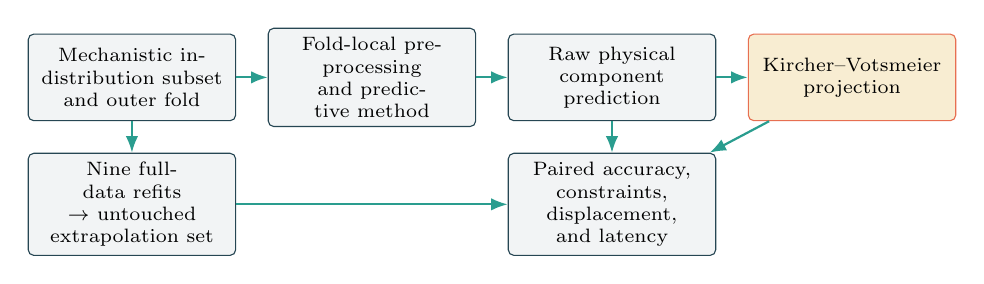
\begin{tikzpicture}[
  node distance=4mm and 4mm,
  flowbox/.style={draw=DeepTeal, rounded corners=2pt, fill=DeepTeal!6,
               text width=24mm, minimum height=11mm, align=center, font=\scriptsize},
  proj/.style={flowbox, fill=MutedAmber!30, draw=CoralRust},
  arrow/.style={-{Latex[length=2.1mm]}, thick, draw=MineralGreen}
]
\node[flowbox] (data) {Mechanistic in-distribution subset\\and outer fold};
\node[flowbox, right=of data] (model) {Fold-local preprocessing\\and predictive method};
\node[flowbox, right=of model] (raw) {Raw physical\\component prediction};
\node[proj, right=of raw] (project) {Kircher--Votsmeier\\projection};
\node[flowbox, below=of raw] (score) {Paired accuracy, constraints,\\displacement, and latency};
\draw[arrow] (data) -- (model);
\draw[arrow] (model) -- (raw);
\draw[arrow] (raw) -- (project);
\draw[arrow] (raw) -- (score);
\draw[arrow] (project) -- (score);
\node[flowbox, below=of data] (ood) {Nine full-data refits\\$\rightarrow$ untouched extrapolation set};
\draw[arrow] (data) -- (ood);
\draw[arrow] (ood) -- (score);
\end{tikzpicture}
\caption{Evaluation workflow linking nested in-distribution cross-validation, paired raw/projected scoring, and external out-of-distribution validation.}
\label{fig:evaluation_workflow}
\end{figure}

\subsection{Evaluation Metrics and Comparative Analysis}

Component-space accuracy is primary because the 20 effluent components are the supervised targets and the physical constraints act before aggregation. To prevent large-scale components from dominating a single summary, the residual for validation observation $i$ and component $j$ is standardized by the training-fold standard deviation $\sigma_j$,
\begin{equation}
e_{ij}^{(m)}=\frac{\hat c_{ij}^{(m)}-c_{out,ij}}{\sigma_j}.
\end{equation}
For a fold containing $n$ observations, the component-standardized mean squared error (nMSE), root mean squared error (nRMSE), and mean absolute error (nMAE) are
\begin{equation}
\mathrm{nMSE}=\frac{1}{20n}\sum_{i=1}^{n}\sum_{j=1}^{20}e_{ij}^{2},\qquad
\mathrm{nRMSE}=\sqrt{\mathrm{nMSE}},\qquad
\mathrm{nMAE}=\frac{1}{20n}\sum_{i=1}^{n}\sum_{j=1}^{20}|e_{ij}|.
\end{equation}
The coefficient of determination ($R^2$) is calculated separately for each component and then averaged with equal component weight. The standard deviations $\sigma_j$ are population standard deviations (denominator equal to the training-row count); a zero-variance training target invalidates the run. The same formulas are applied to raw and projected predictions. Component-specific errors in physical units and secondary metrics for the four reported water-quality quantities are retained for interpretation rather than mixed into the standardized primary score. Across outer folds, every reported metric is summarized descriptively as the five-fold mean $\pm$ sample SD; no hypothesis tests or inferential rank claims are applied.

Physical admissibility is assessed for every component vector using
\begin{equation}
\label{eq:physical_residuals}
v_{mc,i}(c)=\left\|Ac-b_i\right\|_2,\qquad
v_{nn,i}^{*}(c)=\left\|\min(c\oslash\sigma,0)\right\|_1.
\end{equation}
A mass-conservation violation is recorded when $v_{mc,i}>\tau$; a non-negativity violation is recorded when any component is below $-\tau$. Mean, median, maximum, and sample frequency are retained because a small average can conceal rare large violations. The paired accuracy effect and component displacement are
\begin{equation}
\Delta\mathrm{nRMSE}_{m,N}=\mathrm{nRMSE}_{proj,m,N}-\mathrm{nRMSE}_{raw,m,N},\qquad
d_{c,i}^{*,(m)}=\left\|\left(\tilde c_i^{(m)}-c_{raw,i}^{(m)}\right)\oslash\sigma\right\|_2.
\end{equation}
Here $\oslash$ denotes elementwise division and $\sigma$ is the vector of training-fold component standard deviations. Negative $\Delta\mathrm{nRMSE}$ denotes an accuracy benefit from projection; positive values denote a cost. Physical-unit, per-component negative magnitudes and displacements are also retained as secondary diagnostics.

Wall-clock timing is partitioned into preprocessing and model fitting, raw batch inference, projection alone, and end-to-end projected inference. Hyperparameter search time is reported separately. The timing protocol constructs a deterministic 512-row timing set by cycling through the outer validation inputs, thereby holding the number of scored rows constant even when a fold contains fewer than 512 unique observations. Five warm-up calls precede 30 repetitions for each timed path. The median 512-row latency within a fold is divided by 512 and reported in milliseconds per sample; the five fold medians are then summarized as the arithmetic mean $\pm$ sample SD. Projection timing includes scaling, the weighted solve, feasibility checks, and positivity backtracking.

\begin{table}[htbp]
\centering
\caption{Metrics used to compare raw and Kircher--Votsmeier-projected surrogate predictions.}
\label{tab:evaluation_metrics}
\scriptsize
\setlength{\tabcolsep}{3pt}
\begin{tabular}{p{2.3cm}p{3.5cm}p{2.4cm}p{2.4cm}}
\hline
Metric & Definition & Computed on & Interpretation \\
\hline
nMSE & Mean squared standardized component error & 20 ASM components & Penalizes large standardized errors \\
nRMSE & Square root of nMSE & 20 ASM components & Primary accuracy score \\
nMAE & Mean absolute standardized component error & 20 ASM components & Robust average standardized deviation \\
$R^2$ & Equal-weight macro-average of component $R^2$ & 20 ASM components & Explained component variation \\
$v_{mc}$ & $\|Ac-b_i\|_2$ & ASM components & Magnitude of conservation residual \\
$v_{nn}^{*}$ & $\|\min(c\oslash\sigma,0)\|_1$ & Standardized ASM components & Magnitude of negative concentration violations \\
Violation frequency & Percent of samples exceeding $\tau=10^{-10}$ & ASM components & Frequency of infeasible predictions \\
$\Delta$nRMSE & Projected nRMSE minus raw nRMSE & Paired fold predictions & Accuracy benefit ($<0$) or cost ($>0$) \\
$d_c^{*,(m)}$ & $\|(\tilde c^{(m)}-c_{raw}^{(m)})\oslash\sigma\|_2$ & Standardized ASM components & Size of component-space correction \\
Preparation time & Preprocessing plus fit or context construction, excluding search & Training fold & Model preparation cost \\
Inference latency & Raw, projection-only, and end-to-end time & Validation batch & Deployment cost \\
\hline
\end{tabular}
\end{table}

\subsection{Out-of-Distribution Extrapolation Design}

After cross-validation, one final setting per model is selected by a four-fold search that uses only the 10,000 in-distribution states and the same objective and search budget. Each model and its preprocessing are then refitted on the complete in-distribution pool before any OOD target is accessed.

The OOD validation set is generated with new mechanistic simulations. No OOD response is used for refitting, scaling, calibration, or model selection. Four influential inputs are perturbed beyond their configured maxima, while the remaining inputs stay inside their original ranges. Mild excursions have normalized distance $(x_j-U_j)/(U_j-L_j)$ between 0.10 and 0.25; severe excursions have distance between 0.35 and 0.60. Candidate generation targets a 70\% one-variable and 30\% two-variable mixture; realized candidate and accepted-set proportions are reported separately. Every retained point is therefore outside the in-distribution hyperrectangle and, consequently, outside the convex hull of the training data. OOD standardized errors use the population standard deviations of all 10,000 in-distribution targets.

\begin{table}[htbp]
\centering
\caption{Planned out-of-distribution (OOD) input intervals. Values are fixed design bounds, not illustrative performance results.}
\label{tab:ood_domain}
\scriptsize
\begin{tabular}{lllll}
\toprule
Input & In-distribution interval & Mild extrapolation interval & Severe extrapolation interval & Unit \\
\midrule
HRT & $[6,36]$ & $[39,43.5]$ & $[46.5,54]$ & h \\
Aeration & $[0.5,2.5]$ & $[2.7,3.0]$ & $[3.2,3.7]$ & -- \\
$S_{NH4}$ & $[12,55]$ & $[59.3,65.8]$ & $[70.1,80.8]$ & g N/m$^3$ \\
$X_S$ & $[60,280]$ & $[302,335]$ & $[357,412]$ & g COD/m$^3$ \\
\bottomrule
\end{tabular}
\end{table}

The target is 600 accepted steady states per severity band. The same solver, initialization sequence, and residual acceptance rule used for in-distribution generation are retained, and attempted, failed, and accepted counts are reported. OOD comparison uses nMSE, nRMSE, nMAE, physical violation magnitudes and rates, and projection displacement on identical raw/projected sample pairs. The coefficient of determination is secondary because a deliberately shifted response distribution changes its denominator. Structural feasibility and predictive extrapolation are interpreted separately.

\subsection{Computational Environment and Reproducibility}

All pseudorandom operations use seed 42 and preserve the shared subset and fold indices. Double precision is used for mechanistic states, invariant construction, projection, and metrics. The final report will identify the processor, memory, operating system, package versions, and thread limits. Timing values are specific to the accepted workstation and batching protocol and are not transferable performance measurements.

\section{Results and Discussion}

\subsection{Benchmark Dataset and Invariant Verification}

The boxed notice before the Nomenclature applies to every numerical result in this section. The illustrative acceptance profile in Table~\ref{tab:illustrative_dataset_validation} contains the planned 10,000 in-distribution states and 1,200 out-of-distribution states. Acceptance decreases with extrapolation severity, showing why rejected mechanistic simulations must be reported: they narrow the region over which a surrogate can be validated. The illustrative ground-truth states satisfy the declared conservation and non-negativity tolerances, while the unrounded invariant basis gives $\max|A\nu^T|=4.25\times10^{-16}$. Later violation counts therefore diagnose surrogate predictions rather than an inconsistent reference set.

\begin{table}[htbp]
\centering
\caption{Illustrative placeholder---not experimental data: dataset acceptance and ground-truth validation summary. Replace all marked results before submission.}
\label{tab:illustrative_dataset_validation}
\scriptsize
\begin{tabular}{lrrrrr}
\toprule
Set & Attempted & Accepted & Acceptance (\%) & Maximum $v_{mc}$ & Minimum component \\
\midrule
In-distribution & 10,384\illustrative & 10,000 & 96.3\illustrative & $7.6\times10^{-11}$\illustrative & $1.0\times10^{-8}$\illustrative \\
Mild out-of-distribution & 618\illustrative & 600 & 97.1\illustrative & $8.0\times10^{-11}$\illustrative & $1.0\times10^{-8}$\illustrative \\
Severe out-of-distribution & 656\illustrative & 600 & 91.5\illustrative & $8.8\times10^{-11}$\illustrative & $1.0\times10^{-8}$\illustrative \\
\bottomrule
\end{tabular}
\end{table}

\subsection{Planned Primary Demonstration of Simultaneous Physical Enforcement}

Simultaneous physical enforcement is the primary result that the benchmark is designed to test. In the illustrative profile, every surrogate produces a nonzero conservation residual before correction, and 3.2--15.0\% of full-size predictions contain at least one negative component. After the Kircher--Votsmeier projection and selective positivity backtracking, every paired prediction satisfies both requirements within the declared numerical tolerance. Table~\ref{tab:illustrative_projection} later reports the model-level values, while Figure~\ref{fig:illustrative_projection_delta} shows the associated change in predictive error across data sizes.

If verified by the final outputs, this pattern will demonstrate the contribution that is independent of any model leaderboard: one post-prediction procedure can place heterogeneous tabular outputs under the same physical contract without retraining or redesigning the predictor. To our knowledge, that would provide the first such demonstration for activated-sludge tabular surrogates. The nine learners test compatibility across several established model classes.

\subsection{In-Distribution Accuracy and Computational Efficiency}

The complete full-scale benchmark will replace this paragraph with the nine-model five-fold accuracy and training-time findings. Close fold summaries will be treated descriptively and will not be presented as an inferential ordering.

The complete timing analysis will distinguish hyperparameter search, fitting, raw inference, projection, and end-to-end projected inference. All latency values will represent a complete 20-component prediction.

\begin{table}[htbp]
\centering
\caption{Illustrative placeholder---not experimental data: full-size raw in-distribution performance and timing (descriptive five-fold mean $\pm$ sample SD).}
\label{tab:illustrative_full_benchmark}
\scriptsize
\resizebox{\textwidth}{!}{%
\begin{tabular}{lrrrrrr}
\toprule
Model & nRMSE & nMSE & nMAE & Macro-$R^2$ & Fit/setup (s) & Raw latency (ms/sample) \\
\midrule
XGBoost & $.112\pm.007$ & $.0126\pm.0016$ & $.071\pm.004$ & $.974\pm.004$ & $2.80\pm.20$ & $.014\pm.003$ \\
LightGBM & $.106\pm.006$ & $.0113\pm.0013$ & $.067\pm.004$ & $.976\pm.003$ & $1.60\pm.10$ & $.010\pm.002$ \\
CatBoost & $.109\pm.006$ & $.0119\pm.0013$ & $.069\pm.004$ & $.975\pm.003$ & $3.40\pm.20$ & $.017\pm.003$ \\
AdaBoost & $.178\pm.013$ & $.0318\pm.0046$ & $.113\pm.008$ & $.933\pm.006$ & $6.80\pm.40$ & $.085\pm.006$ \\
Random Forest & $.132\pm.009$ & $.0175\pm.0024$ & $.084\pm.006$ & $.964\pm.004$ & $5.50\pm.30$ & $.062\pm.005$ \\
SVR & $.145\pm.009$ & $.0211\pm.0026$ & $.092\pm.006$ & $.956\pm.004$ & $31.0\pm1.70$ & $.240\pm.012$ \\
$k$-NN & $.158\pm.011$ & $.0251\pm.0035$ & $.100\pm.007$ & $.948\pm.005$ & $.05\pm.01$ & $.310\pm.015$ \\
PLS & $.205\pm.008$ & $.0421\pm.0033$ & $.130\pm.005$ & $.911\pm.004$ & $.12\pm.01$ & $.004\pm.001$ \\
MLP & $.120\pm.010$ & $.0145\pm.0024$ & $.076\pm.006$ & $.970\pm.005$ & $18.5\pm2.10$ & $.018\pm.004$ \\

\bottomrule
\end{tabular}}
\parbox{0.96\textwidth}{\scriptsize $^{a}$Context preparation, not conventional parameter fitting. All values are illustrative and must be replaced.}
\end{table}

\subsection{Data-Scarcity Scaling and Predictive Stability}

The complete learning-curve analysis will compare all nine models at all eleven nested sample totals and will report five-fold means with sample SD without attributing differences to untested mechanisms.

The completed timing panel will place predictive learning curves and model-training costs on the same sample-size axis while keeping inference latency in the dedicated timing table.

\begin{figure}[htbp]
\centering
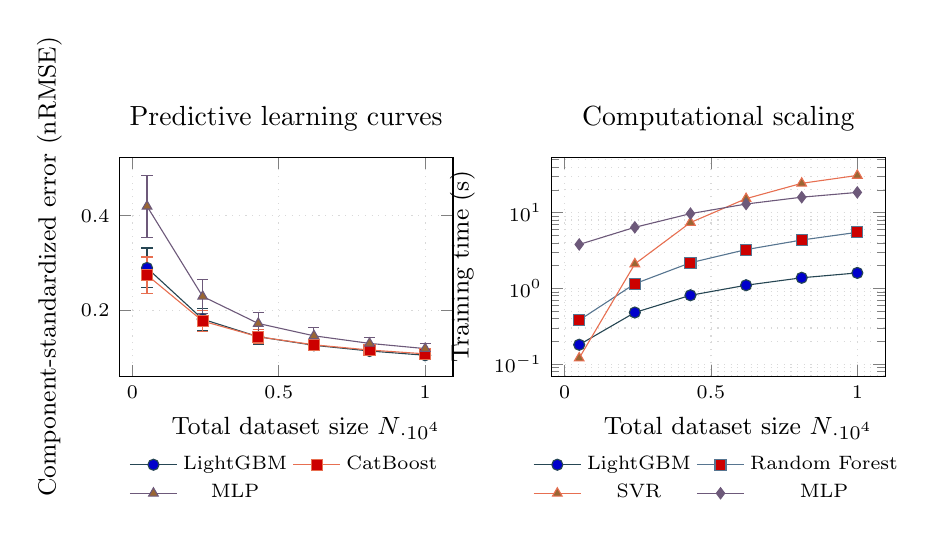
\begin{tikzpicture}
\begin{groupplot}[
 group style={group size=2 by 1, horizontal sep=1.25cm},
 width=0.48\textwidth, height=0.36\textwidth,
 grid=both, grid style={dotted,gray!30},
 tick label style={font=\scriptsize}, label style={font=\small},
 legend style={font=\scriptsize, draw=none, fill=none}
]
\nextgroupplot[
 xlabel={Total dataset size $N$}, ylabel={Component-standardized error (nRMSE)},
 title={Predictive learning curves},
 legend style={at={(0.5,-0.31)},anchor=north,legend columns=2}
]
\addplot+[color=DeepTeal,mark=*,error bars/.cd,y dir=both,y explicit]
 coordinates {(500,.290)+-(0,.042) (2400,.182)+-(0,.023) (4300,.145)+-(0,.016) (6200,.127)+-(0,.011) (8100,.115)+-(0,.008) (10000,.106)+-(0,.006)};
\addlegendentry{LightGBM}
\addplot+[color=CoralRust,mark=square*,error bars/.cd,y dir=both,y explicit]
 coordinates {(500,.275)+-(0,.038) (2400,.178)+-(0,.022) (4300,.145)+-(0,.015) (6200,.128)+-(0,.011) (8100,.117)+-(0,.008) (10000,.109)+-(0,.006)};
\addlegendentry{CatBoost}
\addplot+[color=MutedPlum,mark=triangle*,error bars/.cd,y dir=both,y explicit]
 coordinates {(500,.420)+-(0,.065) (2400,.230)+-(0,.036) (4300,.173)+-(0,.024) (6200,.147)+-(0,.017) (8100,.131)+-(0,.013) (10000,.120)+-(0,.010)};
\addlegendentry{MLP}

\nextgroupplot[
 xlabel={Total dataset size $N$}, ylabel={Training time (s)},
 ymode=log, title={Computational scaling},
 legend style={at={(0.5,-0.31)},anchor=north,legend columns=2}
]
\addplot+[color=DeepTeal,mark=*] coordinates {(500,.18) (2400,.48) (4300,.81) (6200,1.10) (8100,1.38) (10000,1.60)};
\addlegendentry{LightGBM}
\addplot+[color=SteelBlue,mark=square*] coordinates {(500,.38) (2400,1.15) (4300,2.18) (6200,3.25) (8100,4.35) (10000,5.50)};
\addlegendentry{Random Forest}
\addplot+[color=CoralRust,mark=triangle*] coordinates {(500,.12) (2400,2.10) (4300,7.40) (6200,15.3) (8100,24.4) (10000,31.0)};
\addlegendentry{SVR}
\addplot+[color=MutedPlum,mark=diamond*] coordinates {(500,3.8) (2400,6.4) (4300,9.7) (6200,13.0) (8100,16.0) (10000,18.5)};
\addlegendentry{MLP}
\end{groupplot}
\end{tikzpicture}
\caption{Illustrative placeholder---not experimental data: cross-validated nRMSE learning curves (left, descriptive five-fold means with sample-SD bars) and training time (right).}
\label{fig:illustrative_scaling}
\end{figure}

\subsection{Predictive Effect of Physical Enforcement Across Data Sizes}

Table~\ref{tab:illustrative_projection} expands the primary enforcement result by showing how far each raw prediction must move. Raw mass-conservation violation rates are 100\% at the stringent tolerance of $10^{-10}$, so mean residual magnitude is more informative than the count. Standardized projection displacement is smallest for LightGBM and largest for partial least squares in the illustrative profile. Predictive accuracy and distance from the feasible manifold therefore need not rank models identically. The backtracking column also shows that positivity enforcement is activated selectively rather than assumed from scaling alone.

Projection modestly improves full-size nRMSE for nine models in the illustrative values, but partial least squares changes from 0.205 to 0.207. Figure~\ref{fig:illustrative_projection_delta} shows why the full data-scarcity grid matters: the correction provides the largest benefit when raw predictions are least stable, and the benefit contracts as data increase. The partial-least-squares line crosses zero, exemplifying a legitimate accuracy--feasibility tradeoff rather than a failure of structural enforcement.

\begin{table}[htbp]
\centering
\caption{Illustrative placeholder---not experimental data: full-size paired projection ablation. Displayed entries are illustrative fold means only because fold-level placeholder values are unavailable; the final table will report descriptive five-fold mean $\pm$ sample SD. Projected mass and non-negativity violation rates are 0\% for every illustrative row at $\tau=10^{-10}$.}
\label{tab:illustrative_projection}
\scriptsize
\resizebox{\textwidth}{!}{%
\begin{tabular}{lrrrrr}
\toprule
Model & Illustrative mean nRMSE raw $\rightarrow$ projected & Raw non-negativity violation (\%) & Raw mean $v_{mc}$ & Mean $d_c^{*}$ & Backtracking (\%) \\
\midrule
XGBoost & $.112\rightarrow.109$ & 5.2 & .74 & .95 & 4.7 \\
LightGBM & $.106\rightarrow.104$ & 4.0 & .65 & .82 & 3.6 \\
CatBoost & $.109\rightarrow.107$ & 3.5 & .68 & .85 & 3.1 \\
AdaBoost & $.178\rightarrow.171$ & 15.0 & 1.90 & 2.35 & 13.8 \\
Random Forest & $.132\rightarrow.128$ & 6.8 & .95 & 1.22 & 6.1 \\
SVR & $.145\rightarrow.142$ & 10.0 & 1.20 & 1.50 & 9.4 \\
$k$-NN & $.158\rightarrow.153$ & 13.0 & 1.45 & 1.80 & 12.2 \\
PLS & $.205\rightarrow.207$ & 7.0 & 2.10 & 2.70 & 6.4 \\
MLP & $.120\rightarrow.116$ & 7.5 & .82 & 1.05 & 7.0 \\

\bottomrule
\end{tabular}}
\end{table}

\begin{figure}[htbp]
\centering
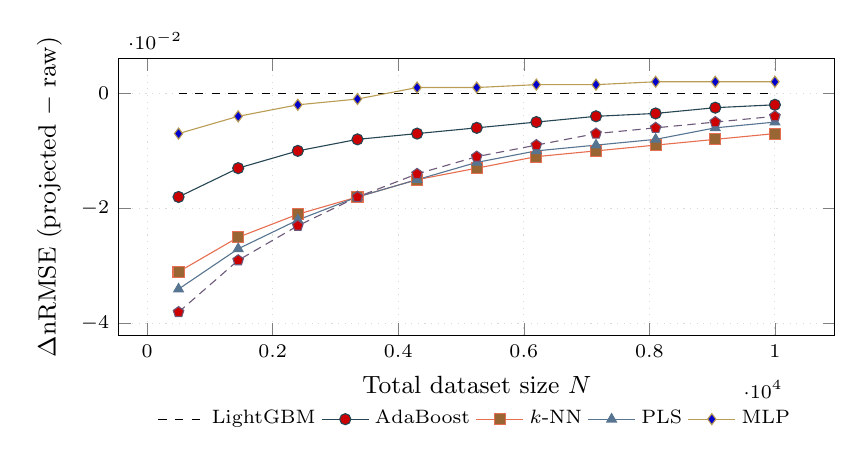
\begin{tikzpicture}
\begin{axis}[
 width=0.88\textwidth,height=0.42\textwidth,
 xlabel={Total dataset size $N$},ylabel={$\Delta$nRMSE (projected $-$ raw)},
 grid=both,grid style={dotted,gray!30},
 tick label style={font=\scriptsize},label style={font=\small},
 legend style={at={(0.5,-0.23)},anchor=north,legend columns=5,font=\scriptsize,draw=none},
]
\addplot[black,dashed,domain=500:10000,samples=2] {0};
\addplot+[color=DeepTeal,mark=*] coordinates {(500,-.018)(1450,-.013)(2400,-.010)(3350,-.008)(4300,-.007)(5250,-.006)(6200,-.005)(7150,-.004)(8100,-.0035)(9050,-.0025)(10000,-.002)};
\addlegendentry{LightGBM}
\addplot+[color=CoralRust,mark=square*] coordinates {(500,-.031)(1450,-.025)(2400,-.021)(3350,-.018)(4300,-.015)(5250,-.013)(6200,-.011)(7150,-.010)(8100,-.009)(9050,-.008)(10000,-.007)};
\addlegendentry{AdaBoost}
\addplot+[color=SteelBlue,mark=triangle*] coordinates {(500,-.034)(1450,-.027)(2400,-.022)(3350,-.018)(4300,-.015)(5250,-.012)(6200,-.010)(7150,-.009)(8100,-.008)(9050,-.006)(10000,-.005)};
\addlegendentry{$k$-NN}
\addplot+[color=MutedAmber!80!black,mark=diamond*] coordinates {(500,-.007)(1450,-.004)(2400,-.002)(3350,-.001)(4300,.001)(5250,.001)(6200,.0015)(7150,.0015)(8100,.002)(9050,.002)(10000,.002)};
\addlegendentry{PLS}
\addplot+[color=MutedPlum,mark=pentagon*] coordinates {(500,-.038)(1450,-.029)(2400,-.023)(3350,-.018)(4300,-.014)(5250,-.011)(6200,-.009)(7150,-.007)(8100,-.006)(9050,-.005)(10000,-.004)};
\addlegendentry{MLP}
\end{axis}
\end{tikzpicture}
\caption{Illustrative placeholder---not experimental data: paired change in nRMSE after projection. Coordinates are illustrative fold means only because fold-level placeholder values are unavailable; the final figure will show descriptive five-fold means with sample-SD bars. Negative values indicate an accuracy benefit; projected constraint violations are zero within tolerance at every displayed point.}
\label{fig:illustrative_projection_delta}
\end{figure}

\subsection{Extrapolation Beyond the Training Domain}

The illustrative out-of-distribution profile contains 600 accepted states in each severity band. Accuracy deteriorates for every model relative to full-size in-distribution validation, and severe excursions alter the displayed ordering (Table~\ref{tab:illustrative_ood}). LightGBM has the lowest displayed raw nRMSE among the tree ensembles under severe shift (0.405). Across all methods, support vector regression and partial least squares have lower displayed raw values of 0.362 and 0.352. After projection, support vector regression has the lowest displayed severe-shift value (0.346), because partial least squares incurs a small correction cost, increasing from 0.352 to 0.361. This illustrative ordering change shows why interpolation performance should not be used as a proxy for extrapolation.

The structural conclusion is more general than the ranking. Projection keeps every illustrative output within the declared conservation and non-negativity tolerances across both extrapolation bands. Before correction, negative-state violations increase with severity, reaching 55\% for $k$-nearest neighbors and 51\% for Adaptive Boosting. Physical admissibility does not, however, make every projected state close to the mechanistic target. Figure~\ref{fig:illustrative_ood} shows that severe-shift nRMSE can improve, remain similar, or worsen, depending on how the raw error aligns with infeasible directions.

\begin{table}[htbp]
\centering
\caption{Illustrative placeholder---not experimental data: raw-to-projected out-of-distribution nRMSE and raw non-negativity violation rates. All projected violation rates are 0\% within tolerance.}
\label{tab:illustrative_ood}
\scriptsize
\resizebox{\textwidth}{!}{%
\begin{tabular}{lrrrr}
\toprule
Model & Mild nRMSE raw $\rightarrow$ projected & Severe nRMSE raw $\rightarrow$ projected & Raw non-negativity mild (\%) & Raw non-negativity severe (\%) \\
\midrule
XGBoost & $.205\rightarrow.196$ & $.430\rightarrow.397$ & 11 & 29 \\
LightGBM & $.198\rightarrow.190$ & $.405\rightarrow.372$ & 9 & 25 \\
CatBoost & $.201\rightarrow.193$ & $.418\rightarrow.384$ & 8 & 23 \\
AdaBoost & $.340\rightarrow.316$ & $.690\rightarrow.623$ & 27 & 51 \\
Random Forest & $.246\rightarrow.232$ & $.515\rightarrow.470$ & 14 & 34 \\
SVR & $.238\rightarrow.229$ & $.362\rightarrow.346$ & 18 & 36 \\
$k$-NN & $.315\rightarrow.291$ & $.642\rightarrow.574$ & 24 & 55 \\
PLS & $.278\rightarrow.281$ & $.352\rightarrow.361$ & 12 & 22 \\
MLP & $.226\rightarrow.210$ & $.448\rightarrow.401$ & 16 & 41 \\

\bottomrule
\end{tabular}}
\end{table}

\begin{figure}[htbp]
\centering
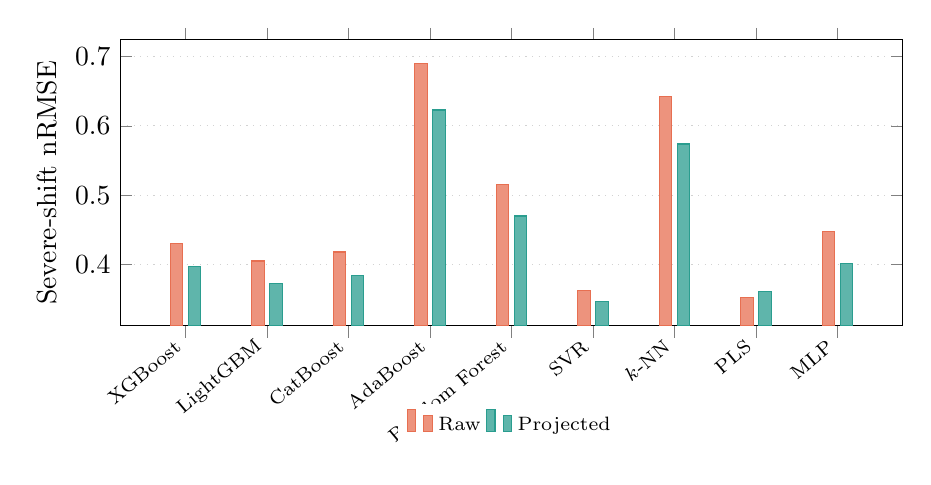
\begin{tikzpicture}
\begin{axis}[
 ybar,bar width=4.5pt,
 width=0.95\textwidth,height=0.43\textwidth,
 ylabel={Severe-shift nRMSE},
 symbolic x coords={xgb,lgbm,cat,ada,rf,svr,knn,pls,mlp},
 xtick=data,xticklabels={XGBoost,LightGBM,CatBoost,AdaBoost,Random Forest,SVR,$k$-NN,PLS,MLP},
 x tick label style={rotate=40,anchor=east,font=\scriptsize},
 ymajorgrids,grid style={dotted,gray!35},
 legend style={at={(0.5,-0.27)},anchor=north,legend columns=2,font=\scriptsize,draw=none},
]
\addplot[fill=CoralRust!75,draw=CoralRust] coordinates {(xgb,.430)(lgbm,.405)(cat,.418)(ada,.690)(rf,.515)(svr,.362)(knn,.642)(pls,.352)(mlp,.448)};
\addlegendentry{Raw}
\addplot[fill=MineralGreen!75,draw=MineralGreen] coordinates {(xgb,.397)(lgbm,.372)(cat,.384)(ada,.623)(rf,.470)(svr,.346)(knn,.574)(pls,.361)(mlp,.401)};
\addlegendentry{Projected}
\end{axis}
\end{tikzpicture}
\caption{Illustrative placeholder---not experimental data: severe out-of-distribution raw and projected nRMSE. Projection restores physical admissibility in the example but does not uniformly improve predictive accuracy.}
\label{fig:illustrative_ood}
\end{figure}

\subsection{Cross-Model Synthesis, Implications, and Limitations}

Taken together, the illustrative values demonstrate the intended decision process rather than a completed model ranking. More importantly, they show how the final benchmark will evaluate the paper's primary contribution: whether the same Kircher--Votsmeier layer removes both declared physical violations across heterogeneous tabular predictors without retraining them. Its illustrative absolute latency is small, although its final relative cost will depend on the speed of the underlying predictor. The placeholders also show how enforcement could improve prediction error when part of a raw residual lies in infeasible directions, while the partial-least-squares example shows how exact feasibility could instead carry a modest accuracy cost.



The extrapolation comparison sets another boundary on the claim. A projected state can conserve mass and remain non-negative while still differing from the mechanistic solution. The method is therefore a common physical contract for surrogate-assisted screening, optimization, and monitoring, not a substitute for predictive-distribution assessment or mechanistic validation beyond the sampled domain.

The planned evidence is simulated and steady state, rather than plant-observed and dynamic. It therefore cannot establish trajectory-wise conservation in an operating treatment plant. Moreover, the five invariants and non-negativity do not imply full kinetic, thermodynamic, or operational feasibility.

Any extrapolation conclusions will depend on the selected exterior intervals and on which mechanistic simulations converge. Computational comparisons will likewise depend on hardware, batching, thread control, search budget, and model configuration. No finite benchmark can cover every machine-learning architecture; the selected learners represent several common model families rather than an exhaustive inventory. Complete fold-level summaries, physical-unit component metrics, extrapolation residual distributions, and fold-specific hyperparameters are provided in the supplementary material after the accepted run.

\FloatBarrier
\section{Conclusion}

To our knowledge, this study aims to provide the first model-agnostic demonstration of simultaneous enforcement of mass conservation and non-negativity across tabular surrogates for an activated-sludge process. Applying the Kircher--Votsmeier correction after prediction is designed to impose one physical contract without retraining or redesigning the underlying model. This planned contribution addresses a requirement that wastewater surrogate studies have largely overlooked even as artificial intelligence and machine-learning tools become more common.

The benchmarking analysis is designed to support that primary contribution by testing nine conventional learners across data scarcity, computational cost, and extrapolation beyond the training range. Most importantly, the study separates two claims: the correction can guarantee mass conservation and non-negativity within numerical tolerance, whereas predictive accuracy remains an empirical property of the learner and the data domain.

The numerical results currently displayed are illustrative placeholders rather than scientific findings. When final outputs replace them, the same paired analysis will quantify the accuracy cost or benefit of enforcement, its computational overhead, and the extent to which raw predictions degrade beyond familiar operating conditions. Those measurements will determine whether the planned activated-sludge demonstration is supported while leaving the mathematical correction mechanism unchanged.

\section*{References}

\noindent Aboagye, E. A., Burnham, S. M., Dailey, J., Zia, R., Tran, C., Desai, M., \& Yenkie, K. M. (2021). Systematic design, optimization, and sustainability assessment for generation of efficient wastewater treatment networks. \textit{Water, 13}(9), 1326. doi: 10.3390/w13091326.

\noindent Ahn, J. Y., Chu, K. H., Yoo, S. S., Mang, J. S., Sung, B. W., \& Ko, K. B. (2014). Determination of optimal operating factors via modeling for livestock wastewater treatment: Comparison of simulated and experimental data. \textit{International Biodeterioration \& Biodegradation, 95}, 46--54. doi: 10.1016/j.ibiod.2014.04.014.

\noindent Asadi, A., Verma, A., Yang, K., \& Mejabi, B. (2017). Wastewater treatment aeration process optimization: A data mining approach. \textit{Journal of Environmental Management, 203}, 630--639. doi: 10.1016/j.jenvman.2016.07.047.

\noindent Bagherzadeh, F., Mehrani, M. J., Basirifard, M., \& Roostaei, J. (2021). Comparative study on total nitrogen prediction in wastewater treatment plant and effect of various feature selection methods on machine learning algorithms performance. \textit{Journal of Water Process Engineering, 41}, 102033. doi: 10.1016/j.jwpe.2021.102033.

\noindent Beucler, T., Pritchard, M., Rasp, S., Ott, J., Baldi, P., \& Gentine, P. (2021). Enforcing analytic constraints in neural networks emulating physical systems. \textit{Physical Review Letters, 126}(9), 098302. doi: 10.1103/PhysRevLett.126.098302.

\noindent Bhosekar, A., \& Ierapetritou, M. (2018). Advances in surrogate based modeling, feasibility analysis, and optimization: A review. \textit{Computers \& Chemical Engineering, 108}, 250--267. doi: 10.1016/j.compchemeng.2017.09.017.

\noindent Duan, S., Zhang, Y., \& Zheng, S. (2022). Heterotrophic nitrifying bacteria in wastewater biological nitrogen removal systems: A review. \textit{Critical Reviews in Environmental Science and Technology, 52}(13), 2302--2338. doi: 10.1080/10643389.2021.1877976.

\noindent Durkin, A., Otte, L., \& Guo, M. (2024). Surrogate-based optimisation of process systems to recover resources from wastewater. \textit{Computers \& Chemical Engineering, 182}, 108584. doi: 10.1016/j.compchemeng.2024.108584.

\noindent Fuck, J. V. R., Cechinel, M. A. P., Neves, J., de Andrade, R. C., Trist\~ao, R., Spogis, N., Riella, H. G., Soares, C., \& Padoin, N. (2024). Predicting effluent quality parameters for wastewater treatment plant: A machine learning-based methodology. \textit{Chemosphere, 352}, 141472. doi: 10.1016/j.chemosphere.2024.141472.

\noindent Guerrero, J., Guisasola, A., \& Baeza, J. A. (2011). The nature of the carbon source rules the competition between PAO and denitrifiers in systems for simultaneous biological nitrogen and phosphorus removal. \textit{Water Research, 45}(16), 4793--4802. doi: 10.1016/j.watres.2011.06.019.

\noindent Hansen, D., Maddix, D. C., Alizadeh, S., Gupta, G., \& Mahoney, M. W. (2024). Learning physical models that can respect conservation laws. \textit{Physica D: Nonlinear Phenomena, 457}, 133952. doi: 10.1016/j.physd.2023.133952.

\noindent Henze, M., Gujer, W., Mino, T., \& van Loosdrecht, M. (2006). Activated Sludge Models ASM1, ASM2, ASM2d and ASM3. \textit{Water Intelligence Online, 5}(0). doi: 10.2166/9781780402369.





\noindent Kim, M., Rao, A. S., \& Yoo, C. (2009). Dual optimization strategy for N and P removal in a biological wastewater treatment plant. \textit{Industrial and Engineering Chemistry Research, 48}(13), 6363--6371. doi: 10.1021/ie801689t.

\noindent Kircher, T., \& Votsmeier, M. (2025). Machine learning surrogate models for mechanistic kinetics: Embedding atom balance and positivity. \textit{The Journal of Physical Chemistry Letters, 16}(19), 4715--4723. doi: 10.1021/acs.jpclett.5c00602.

\noindent Li, M., Hu, S., Xia, J., Wang, J., Song, X., \& Shen, H. (2020). Dissolved oxygen model predictive control for activated sludge process model based on the fuzzy C-means cluster algorithm. \textit{International Journal of Control, Automation and Systems, 18}(9), 2435--2444. doi: 10.1007/s12555-019-0438-1.

\noindent Lim, J., Lee, Y., Ataei, A., \& Yoo, C. (2011). Exploration of dual optimal conditions for COD and nitrogen removal in an MBR. \textit{Asia-Pacific Journal of Chemical Engineering, 6}(3), 433--440. doi: 10.1002/apj.563.

\noindent Lin, L., Yang, H., \& Xu, X. (2022). Effects of water pollution on human health and disease heterogeneity: A review. \textit{Frontiers in Environmental Science, 10}, 880246. doi: 10.3389/fenvs.2022.880246.



\noindent Madhav, S., Ahamad, A., Singh, A. K., Kushawaha, J., Chauhan, J. S., Sharma, S., \& Singh, P. (2019). Water pollutants: Sources and impact on the environment and human health. In \textit{Sensors in water pollutants monitoring: Role of material} (pp. 43--62). doi: 10.1007/978-981-15-0671-0\_4.

\noindent Mao, Z., Li, X., Zhang, X., Li, D., Lu, J., Li, J., \& Zheng, F. (2024). Optimization of effluent quality and energy consumption of aeration process in wastewater treatment plants using artificial intelligence. \textit{Journal of Water Process Engineering, 63}, 105384. doi: 10.1016/j.jwpe.2024.105384.

\noindent Min, Y., Sonar, A., \& Azizan, N. (2024). Hard-constrained neural networks with universal approximation guarantees. \textit{arXiv preprint arXiv:2410.10807}.

\noindent Padron-Paez, J. I., Almaraz, S. D. L., \& Rom\'an-Mart\'inez, A. (2020). Sustainable wastewater treatment plants design through multiobjective optimization. \textit{Computers \& Chemical Engineering, 140}, 106850. doi: 10.1016/\allowbreak j.compchemeng.\allowbreak 2020.\allowbreak 106850.



\noindent Raissi, M., Perdikaris, P., \& Karniadakis, G. E. (2019). Physics-informed neural networks: A deep learning framework for solving forward and inverse problems involving nonlinear partial differential equations. \textit{Journal of Computational Physics, 378}, 686--707. doi: 10.1016/j.jcp.2018.10.045.

\noindent Sturm, P. M., Cappa, C. D., \& Wexler, A. S. (2023). Advecting superspecies: Efficiently modeling transport of organic aerosol with a mass-conserving dimensionality reduction method. \textit{Journal of Advances in Modeling Earth Systems, 15}(3), e2022MS003235. doi: 10.1029/2022MS003235.

\noindent Sturm, P. M., \& Silva, S. J. (2025). A nudge to the truth: Atom conservation as a hard constraint in models of atmospheric composition using a species-weighted correction. \textit{ACS ES\&T Air, 5}(1), 279--289. doi: 10.1021/acsestair.4c00220.

\noindent Sturm, P. M., \& Wexler, A. S. (2020). A mass- and energy-conserving framework for using machine learning to speed computations: A photochemistry example. \textit{Geoscientific Model Development, 13}(9), 4435--4442. doi: 10.5194/gmd-13-4435-2020.

\noindent Sturm, P. M., \& Wexler, A. S. (2022). Conservation laws in a neural network architecture: Enforcing the atom balance of a Julia-based photochemical model (v0.2.0). \textit{Geoscientific Model Development, 15}(9), 3417--3431. doi: 10.5194/gmd-15-3417-2022.

\noindent Tsochatzidi, A., Cenci, F., Aroniada, M., \& Papageorgiou, L. G. (2025). A novel surrogate-based optimisation framework for pharmaceutical process systems. \textit{International Journal of Pharmaceutics, 682}, 125861. doi: 10.1016/j.ijpharm.2025.125861.

\noindent Utkarsh, Maddix, D. C., Ma, R., Mahoney, M. W., \& Wang, Y. (2025). End-to-end probabilistic framework for learning with hard constraints. \textit{arXiv preprint}.

\noindent Wang, Y., Li, T., Bai, L., Yu, H., \& Qu, F. (2025). Comparison of interpretable machine learning models and mechanistic model for predicting effluent nitrogen in WWTP. \textit{Journal of Water Process Engineering, 77}, 108344. doi: 10.1016/j.jwpe.2025.108344.

\noindent Xiao, Y., Zhao, B., Zhang, X., \& Yue, X. (2025). A new paradigm in activated sludge management: An interpretable framework integrating mechanistic dynamics with a data-driven surrogate model. \textit{Environmental Research}, 123435. doi: 10.1016/j.envres.2025.123435.

\noindent Yang, T., Qiu, W., Ma, Y., Chadli, M., \& Zhang, L. (2014). Fuzzy model-based predictive control of dissolved oxygen in activated sludge processes. \textit{Neurocomputing, 136}, 88--95. doi: 10.1016/j.neucom.2014.01.025.

\noindent Yang, S. J., Kim, J., Eom, J., Kim, M., Lee, M., \& Lee, K. H. (2025). Machine learning based prediction of waste activated sludge generation for optimization of WWTP operational efficiency. \textit{Environmental Research}, 122990. doi: 10.1016/j.envres.2025.122990.

\end{document}
